\documentclass[letterpaper,12pt,fleqn]{article}
\usepackage{matharticle}
\usepackage{graphicx}
\pagestyle{plain}
\begin{document}

\begin{center}
\Large Math-08 Homework \#9 Solutions
\end{center}

\vspace{0.5in}

\underline{Reading}

\begin{itemize}
\item Text book section 2.1
\end{itemize}

\underline{Problems}

Consider the equation $y=x^2-1$
\begin{enumerate}
\item Find the $x$-intercepts (if any).

  To find $x$-intercepts, we set $y$ to 0:
  \[0=x^2-1\]
  \[x^2=1\]
  \[x=\pm1\]
  Remember, intercepts are points, so we need to state this answer as
  follows:
  \[(\pm1,0)\]
  
\item Find the $y$-intercepts (if any).

  To find $y$-intercepts, we set $x$ to 0:
  \[y=0^2-1=-1\]
  \[(0,-1)\]

\item Test for symmetry (remember to show all three tests).

  To test for $x$-axis symmetry, we replace $y$ with $-y$ and see if we get
  the same equation back:
  \[-y=x^2-1\]
  \[y=-x^2+1\ne x^2-1\]
  No $x$-axis symmetry.

  To test for $y$-axis symmetry, we replace $x$ with $-x$ and see if we get
  the same equation back:
  \[y=(-x)^2-1=x^2+1\]
  Has $y$-axis symmetry.

  To test for origin symmetry, we replace both $x$ and $y$:
  \[-y=(-x)^2-1\]
  \[y=-x^2+1\ne x^2-1\]
  No origin symmetry.

\item Using you calculator, graph the equation and use the ``zero'' function
  to determine the $x$-intercepts. Turn in screenshots showing the
  identification of each intercept.

  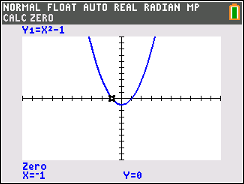
\includegraphics{hw11-4-1}

  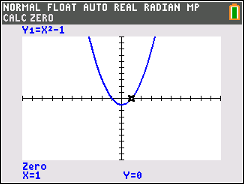
\includegraphics{hw11-4-2}
\end{enumerate}
\end{document}
